%%
%\documentclass[letterpaper, titlepage,openright, twoside,11pt]{book}
%\usepackage[latin1]{inputenc}
%\usepackage{amsmath}
%\usepackage{amsthm}
%\usepackage{amsfonts}
%\usepackage{amssymb}
%\usepackage[spanish]{babel}
%\usepackage[latin1]{inputenc}
%\usepackage{graphicx}
%\usepackage{amsmath}
%\usepackage{dsfont} % colocar los numeros r
%\usepackage{float}
%\usepackage{fancyhdr}
%\usepackage{anysize}
%\decimalpoint
%\begin{document}
%\renewcommand{\tablename}{Tabla}

%\addcontentsline{toc}{chapter} {Elementos Generales de confiabilidad}
%%%%%%%%%%%%%%%%%%%%%%%%%%%%%%%%%%%%
\chapter{Objetivos}

\section{Definici\'on del problema}

\noindent En el 2006 los transformadores de instrumento en las  sub\'areas de Coatzacoalcos y Temascal (Veracruz), observaron un n\'umero inusualmente elevado de fallas, lo que condujo a la necesidad de estudiar la confiabilidad de los transformadores. Se deseaba pronosticar el n\'umero de fallas de sus equipos  por a\~no. En el estudio realizado por el CIMAT, se hizo un an\'alisis de los datos disponibles, empezando por un an\'alisis exploratorio. Posteriormente realizaron distintas comparaciones por tipo, estatus y marca de los transformadores, para  finalmente centrarse en el estudio de los transformadores con m\'as fallas, que resultaron ser los transformadores de corriente. \\[0.1cm]
\noindent Al realizar el an\'alisis de confiabilidad se obtuvo que la distribuci\'on que mejor ajustaba a los datos es una distribuci\'on  Weibull. Bajo esta distribuci\'on se estimaron los par\'ametros, algunos cuantiles de inter\'es e intervalos de confianza usando la aproximaci\'on normal. Adem\'as se analiz\'o el estado de las unidades que sobrevivieron a un tiempo determinado, mediante la funci\'on de riesgo y la confiabilidad condicional, con la finalidad de pronosticar las tasas de falla de los transformadores.\\[0.1cm]

\noindent El inter\'es de este trabajo radica en realizar un an\'alisis de confiabilidad desde el enfoque Bayesiano, hacer estimaciones de las funciones de confiabilidad y describir la tasa de desgaste de las unidades. Esto conducir\'a a proponer una pol\'itica adecuada que minimice los costos de almacenamiento de los equipos, mediante una funci\'on de utilidad, para pronosticar el n\'umero de transformadores requeridos en el almac\'en hasta un tiempo espec\'ifico.


\section{Justificaci\'on}

\noindent Actualmente una de las mayores necesidades de una empresa o negocio, es el empleo \'optimo de sus herramientas de trabajo. Una falla en sus instrumentos implica p\'erdidas en mayor o menor medida. As\'i el implementar pol\'iticas \'optimas y planes estrat\'egicos de sus herramientas de uso, ha significado una parte crucial en el desempe\~no de su trabajo.\\
\noindent Por lo tanto, el generar un plan de inventario para los transformadores resultar\'a de gran importancia. Dado que los transformadores de instrumento son costosos, resultar\'a  \'util estimar su tiempo de vida. \\
%En particular los costos que se  analizar\'an son los siguientes:
%\begin{itemize}
%\item El costo de almacenamiento de los transformadores que no son usados en un periodo dado pero est\'an disponibles en el almac\'en.
%\item El costo de no poder cobrar la electricidad durante un periodo donde no hab\'ia un transformador en reserva.
%\end{itemize}

\noindent La presente investigaci\'on se justifica desde dos puntos de vista:
\begin{itemize}
\item Desde el punto de vista pr\'actico, se desea proponer al problema planteado una estrateg\'ia de acci\'on, empleando funciones de utilidad que permitan minimizar los costos esperados.
\item Desde el punto de vista te\'orico, esta investigaci\'on generar\'a reflexi\'on y discusi\'on sobre el conocimiento existente, en cuanto a la forma de comportarse de los transformadores.
\end{itemize}

\noindent Dentro del desarrollo de esta tesina se har\'a lo siguiente:

\begin{enumerate}
\item Revisar la teor\'ia Bayesiana necesaria para abordar el problema.
\item Proponer alguna estrategia \'optima de inventario o almacenamiento, mediante una funci\'on de utilidad que permita minimizar los costos esperados. 

\end{enumerate}
\noindent A continuaci\'on mencionaremos que son los transformadores de instrumento, y en que radica la importancia en desarrollar un plan \'optimo de inventario.


\section{Transformadores de Instrumento}

\noindent Un transformador el\'ectrico utiliza las propiedades f\'isicas de la inducci\'on electromagn\'etica y es capaz de elevar o disminuir la tensi\'on el\'ectrica, transformar la frecuencia, equilibrar o desequilibrar circuitos el\'ectricos, seg\'un la necesidad y caso espec\'ifico.\\
\noindent El primer transformador fue construido por Michael Faraday, compuesto por dos bobinas enrolladas una encima de la otra. Al variar la corriente que circulaba en una de ellas, cerrando o abriendo el interruptor, el flujo magn\'etico a trav\'es de la otra bobina variaba, y se induc\'ia una corriente el\'ectrica.\\[0.1cm]
\noindent A partir de entonces se han creado diferentes tipos de transformadores cada vez m\'as sofisticados, pero empleando el mismo principio de inducci\'on. En particular en esta tesina se utilizar\'an un tipo especial de transformadores, llamados transformadores de instrumento.\\[0.1cm]
%flujo electromagn�tico, es la medida o cantidad de magnetismo, considerando la intensidad y la extensi�n de un campo magn�tico, un campo magn�tico es un campo de fuerzas que existe alrededor de un campo cuerpo magn�tico o de un conductor que transporta corriente. 
\noindent Los transformadores de instrumento (TI) tienen la tarea de convertir grandes valores de corriente y voltaje a valores peque\~nos que son f\'acilmente aplicables, para los prop\'ositos de medici\'on y protecci\'on. Su misi\'on es evitar la presencia de elevadas tensiones en aquellos dispositivos que van a estar al alcance de las personas. Estos transformadores pueden ser de dos tipos:
\begin{itemize}
\item Transformador de potencial(TP): Cuya funci\'on es transformar o cambiar el voltaje, com\'unmente se enfocan en reducir el voltaje. %,es decir, modera la fuerza con que se mueven los electrones.
\item Transformador de corriente (TC): Su funci\'on consiste en transformar o cambiar la corriente.
%es decir, se encargan de cambiar la cantidad de electrones  que circulan en un determinado momento.
\end{itemize}


%
%Las principales razones por las que se usan los transformadores de instrumento son 
%\begin{itemize}
%\item Para reducir en forma precisa, por medio de la relaci\'on de transformaci\'on, la magnitud de la corriente o voltaje del circuito primario a valores mas manejables en el circuito secundario. Por lo general la salida del secundario a 115 o 120 Volts en el TP y 5 a 1 Amp en el TC.
%\item Para aislar el equipo secundario (instrumentos de medici\'on y de protecci\'on) del voltaje primario, que por su valor los da\~naria.
%\end{itemize}

 \begin{figure}[h!]
\begin{center}
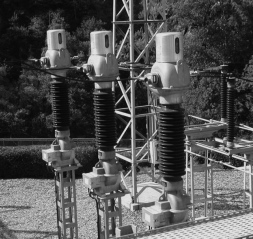
\includegraphics[scale=0.8]{trans.jpg}
\end{center}
\vspace{-.5 cm} \caption{\bf Transformadores de medici\'on.}\label{tranF}
\end{figure}

\noindent Los transformadores resultan de suma importancia en la generaci\'on y distribuci\'on de la energ\'ia el\'ectrica. Su inter\'es principal radica en los siguientes puntos: 

\begin{itemize}
\item Los transformadores de instrumento (Figura\ref{tranF}), ayudan a determinar los consumos de energ\'ia, formando parte del sistema de medici\'on de energ\'ia el\'ectrica para las redes de alta tensi\'on y con ellos realizar los montos de los  cobros. En la parte superior del transformador se conecta la red el\'ectrica. Mientras que en la parte inferior se colocan los elementos de medici\'on, en esta parte la tensi\'on el\'ectrica es mucho m\'as reducida que en la superior.
\item Sirven de protecci\'on, al momento en que se origina una descarga. El sistema designado para protecci\'on desactiva los interruptores, con lo que evita que se generen da\~nos de mayor magnitud en la red.
\item Cuando el transformador falla de manera catastr\'ofica impide la medici\'on del flujo de energia el\'ectrica.
\end{itemize}
\noindent  La falta de alguno de ellos implica p\'erdidas econ\'omicas para la empresa que proveer el servicio de energ\'ia . Sin embargo el tener demasiados en almac\'en implica p\'erdidas tambi\'en. Lo ideal es encontrar  una cantidad adecuada de transformadores, de tal forma que los costo sean m\'inimos, esto es debemos optimizar el inventario.

  

   
  
%  
%  La energ\'ia el\'ectrica en tiempo real son sistemas que sumistran energ\'ia. En tiempo real significa que e la energ\'ia es generada, transformada y suministrada al momento 
%

\newpage \thispagestyle{empty} \cleardoublepage







%\end{document}